\documentclass[12pt]{article}

\usepackage[a4paper,margin=1in]{geometry}
\usepackage{amsmath,amssymb}
\usepackage{enumitem}
\usepackage{graphicx}
\usepackage{multicol}

\begin{document}

\noindent
\begin{minipage}[c]{0.25\textwidth}
    
\includegraphics[width=0.9\linewidth]{iiitb_logo.jpg}
\end{minipage}
\hfill
\begin{minipage}[c]{0.35\textwidth}
    \raggedleft
    \textbf{Name:} Shaik Mansoor\\
    \textbf{ID:} COMETFWC075\\
    \textbf{Date:} \today
\end{minipage}

\vspace{0.2cm}
\hrule
\vspace{0.5cm}

The following Karnaugh map represents a function $F$.

\begin{center}
    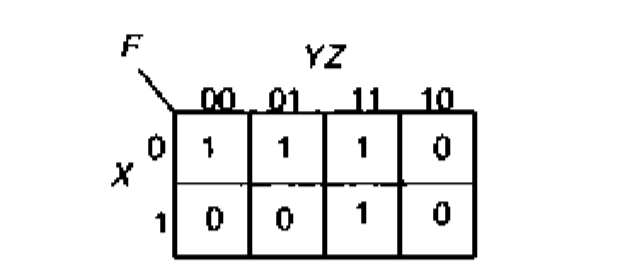
\includegraphics[width=0.4\linewidth]{kmap.png}
\end{center}

\vspace{0.2cm}

Q.52 \hspace{0.2cm} A minimized form of the function $F$ is

\vspace{0.3cm}

\begin{multicols}{2}

\begin{enumerate}[label=(\Alph*)]

\item $
\overline{X}Y + YZ
$

\item[$\checkmark$ (B)] $
\overline{X}\,\overline{Y} + YZ
$

\item $
\overline{X}\,\overline{Y} + Y\overline{Z}
$

\item $
\overline{X}\,\overline{Y} + \overline{Y}Z
$

\end{enumerate}

\end{multicols}

\vspace{0.5cm}

\textbf{Solution:}

From the K-map,

\begin{itemize}

\item The two adjacent 1's in the first row corresponding to 
$YZ=00$ and $YZ=01$ are grouped together.

Here, $X=0$ and $Y=0$ remain constant.

Hence, the term obtained is

$
\overline{X}\,\overline{Y}
$

\item The two 1's in the column corresponding to 
$YZ=11$ are grouped together.

Here, $Y=1$ and $Z=1$ remain constant.

Hence, the term obtained is

$
YZ
$

\end{itemize}

Therefore,

$
F=\overline{X}\,\overline{Y}+YZ
$

Hence, the correct answer is

$
\boxed{(B)}
$

\end{document}


